% \chapter{Fractures}
% \chapter{Introduction}
\begin{figure}[htpb]%
    \centering%
    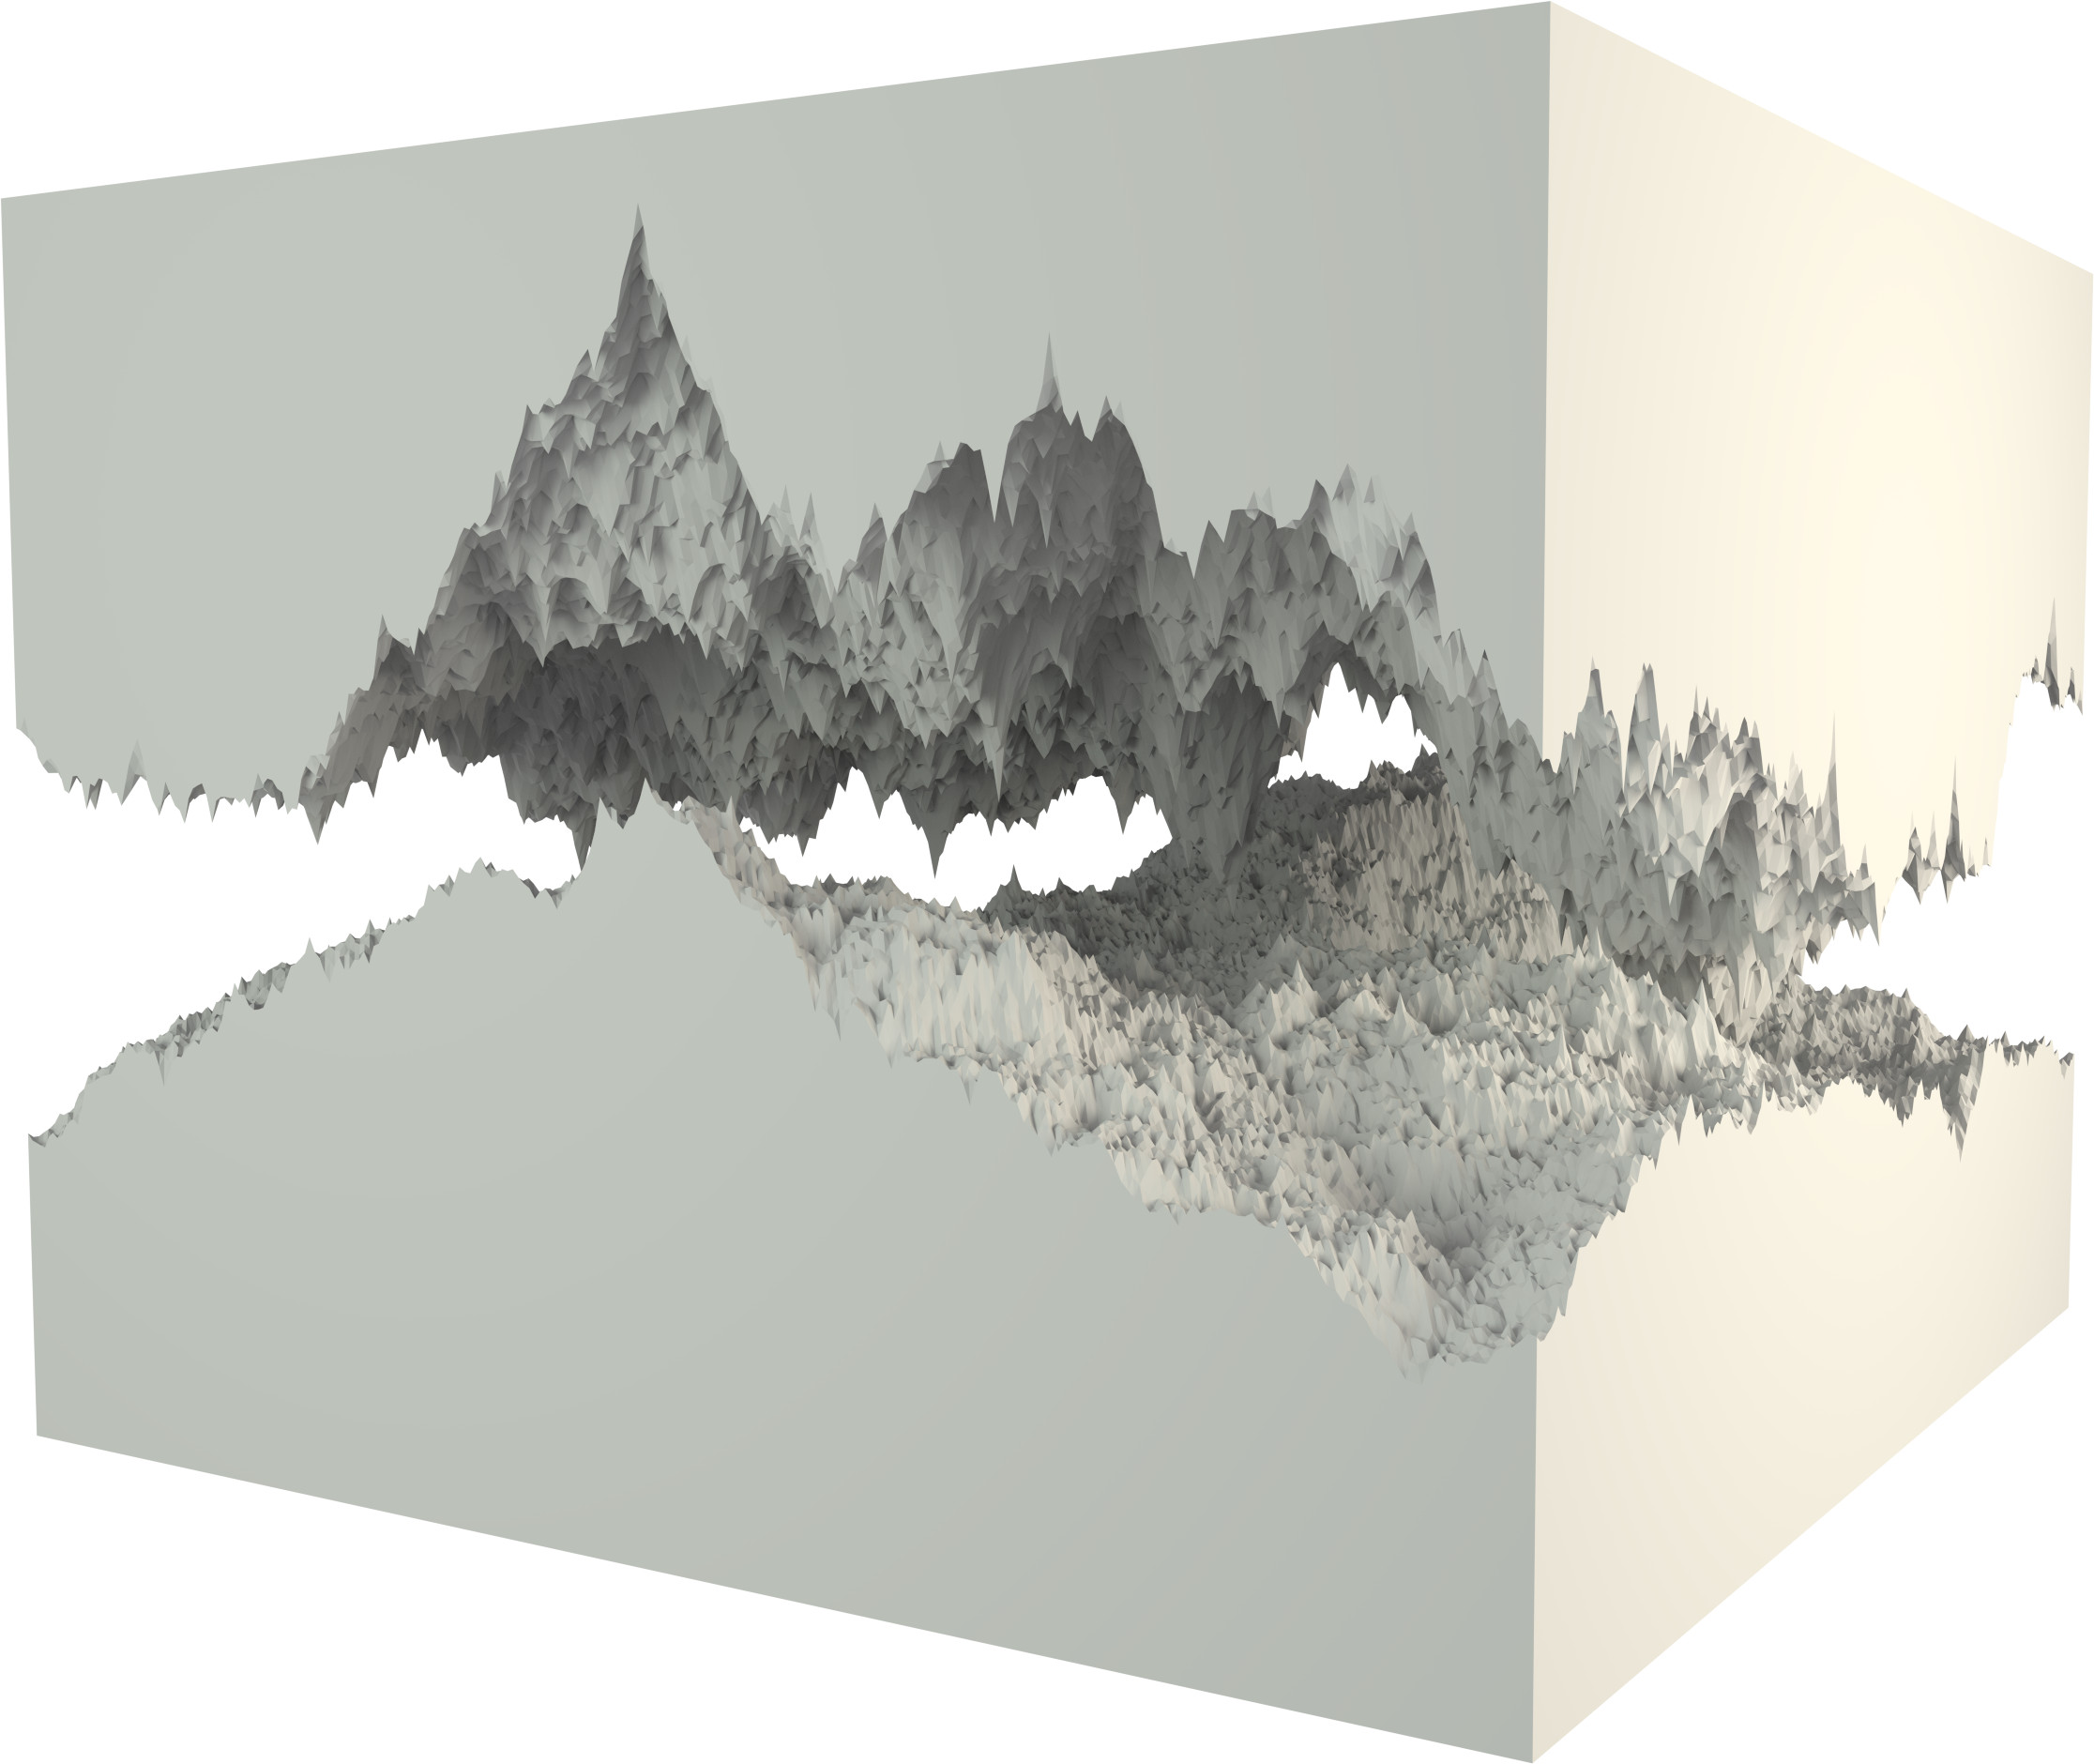
\includegraphics[width=\textwidth]{images/fracture/large_fracture05.jpg}%
    \caption{Caption}%
\end{figure}%

\chapter{Introduction}
We want to study the behaviour of water trapped in nanoscale (pores and) fractures in silica, so need want a way to generate and characterize such a structure. (Several methods of characterizing a fracture could be imagined (\hl{SOURCES, examples}), and we will use several of them.)        

\hl{terrain == heightmap??, finn bra ord her}

\orangebox{
    \begin{itemize}
        \item Plot 1D DMA estimate vs. synthesized 1D fBm from FracLab. Difference between with and without new $f^*$.
        \item Plot 2D DMA estimate vs. synth. 2D fBm from FracLab? \hl{Does FracLab generated 2D?}
        \item Plot 2D DMA est. vs. input Hurst for diamond square. Compare with and without addition and PBC.
    \end{itemize}

}

\chapter{Characterization}

\todo{change wording? copied from Fractals...}
An \emph{affine transformation} transforms a point $\bvec x = (x_1, \dots, x_n)$ into new points $\bvec x' = (r_1x_1, \dots, r_n, x_n)$, where the scaling rations $r_1, \dots, r_n$ are \emph{not} all equal.

A bounded set $\mathcal{S}$ is \emph{self-affine} if $\mathcal{S}$ is the union of $N$ non-overlapping subsets $\mathcal{S}_1, \dots, \mathcal{S}_N$, each of which is congruent to the set $\bvec r(\mathcal{S})$ obtained from $\mathcal S$ by the affine transform defined by $\bvec r$. Here \emph{congruent} means that the set of points $\mathcal{S}$ is identical to the set of points $\bvec r(\mathcal{S})$ after possible translations and/or rotations of the set\cite{feder1988fractals}.

A set $\mathcal{S}$ is \emph{statistically self-affine} if $\mathcal{S}$ is the union of $N$ non-overlapping subsets each of which is scaled down by $\bvec r$ from the original, and is identical in all statistical respects to $\bvec r(\mathcal{S})$.

\section{Hurst exponent}
\orangebox{
\begin{itemize}
    \item define fractal dimension
\end{itemize}
}

One common method to characterize fractals is by the Hurst exponent, usually called $H$\footnote{\todo[inline]{The name used by Hurst in his work where he first describes the exponent was actually $K$\cite{hurst1965longterm}\cite{hurst1951longterm}}}, which comes from a statistical method developed by Hurst\cite{hurst1965longterm}\cite{hurst1951longterm}. The Hurst exponent is related to the fractal dimension $D$ by
\begin{align*}
    D = d-H,
\end{align*}
where $d$ is the spatial dimension of the fractal's domain\cite{feder1988fractals}.

The statistical method developed by Hurst is called \emph{rescaled range analysis} and was designed for use on 1-dimensional time series $f(t)$. The method has been generalized to higher dimensions\cite{fan2013rescaled}, but the original 1D form is shown here.

\todo[inline]{Something about that it's hard to measure, and why.}

\subsection{Rescaled range analysis}
First the time series is divided into \todo{overlapping/non-overlapping?} intervals of length $\tau$. The average over each interval of length $\tau$ is
\begin{align*}
    \langle f \rangle_\tau = \frac{1}{\tau} \sum_{t=1}^\tau f(t).
\end{align*}
We let $F$ be the accumulated deviation from the mean
\begin{align*}
    F(t, \tau) = \sum_{t' = 1}^t \big( f(t') - \langle f \rangle_\tau \big).
\end{align*}
The difference between the maximum and minimum of the accumulated deviation from the mean is the \emph{range} R
\begin{align*}
    R(\tau) = \max_{1 \leq t \leq \tau} \big(F(t,\tau)\big) - \min_{1 \leq t \leq \tau} \big(F(t, \tau)\big).
\end{align*}
The standard deviation $S$ of the time series is estimated using
\begin{align*}
    S^2 = \frac{1}{\tau} \sum_{t=1}^\tau \big( f(t) - \langle f \rangle_\tau \big)^2.
\end{align*}
Hurst found that the observed \emph{rescaled range}, $R/S$, for many time series is described by the \hl{empirical} relation\cite{feder1988fractals}
\begin{align*}
    \frac{R}{S} = \left(\frac{\tau}{2}\right)^H \sim \tau^H.
\end{align*}
We now see that we can estimate the Hurst exponent by a linear fit of the form
\begin{align*}
    \log \left(\frac{R}{S}\right) \sim H\log\tau,
\end{align*}
where we find $H$ as the slope of the linear fit.




\section{Detrending moving average\label{sec:dma}}
\todoa{Plot of $\sigma_\text{DMA}^2$ as function of $n$ to determine $H$}
\todobo{Transition from rescaled range to surface?}
To estimate the Hurst exponent of a surface we use a method called detrending moving average (DMA) developed for 1-dimensional data by E. Alessio, A. Carbone et al.\cite{alessio2002dma}, and later generalized to higher dimensions by A. Carbone \cite{carbone2007algorithm}. 

After trying out some different methods for estimating the Hurst exponent, we ended up choosing this method both because it is \hl{easy} to understand and implement, and because it has been shown to give good results, as we will also confirm later. A more detailed comparison of different methods for estimating the Hurst exponent can be seen in\cite{shao2012comparing}, where they find that DMA and DFA (detrended fluctuation analysis) overall perform better than FA (fluctuation analysis), also being less sensitive to the choice of scaling range.%
\todo{good results, easy to implement? }%
\todoao{everything below is for 2/3 D, not always obvious}%

\subsection{Detrending moving average in 2 dimensions}
% We define a \hl{(self-affine)} surface $f(i,j)$, where $f$ is the height in the point $(i,j)$, defined in a discrete 2-dimensional domain with size $N\times N$, for $i,j = 1,\dots,N$. We divide this surface into \emph{overlapping} subsurfaces of size $n \times n$, spanning the whole surface. The \hl{lower left} corners of the surfaces are located in the points $(i,j)$ for $i,j = 1,\dots, N-n+1$ (the limits are set so that the subsurfaces stay within the domain of the surface). In each surface we find a point $(k,l) = (n-m,n-m)$ (relative to lower bottom corner of subsurface)

We define a \hl{(self-affine)} surface $f(i,j)$ of size $N,N$, with $i,j \in [1,N]$. For each point $i,j \in [1,N-n+1]$ in this surface we define a subsurface of size $n\times n$, where each subsurface consists if the points
\begin{align*}
%     (k,l) = \left([i, \dots, i+n], [j, \dots, j+n]\right)%
%     (k,l) = (i,j) + ([1\dots,n], [1,\dots,n])%
%     (k,l) = (i,j) + \left([1\dots,n], [1,\dots,n]\right) \\
    (k,l) \in \left\{ (i,j) + \left([1\dots,n], [1,\dots,n]\right)\right\}
%     (k,l) \in \left( i + [1\dots,n], j + [1,\dots,n]\right)%
\end{align*}
\begin{align*}
    \begin{pmatrix}
        k \\
        l
    \end{pmatrix}
    =
    \begin{pmatrix}
        i \\
        j
    \end{pmatrix}
    +
    \begin{pmatrix}
        1,\dots,n \\
        1,\dots,n
    \end{pmatrix}
\end{align*}%
\todoao{Decide on which vector/matrix thing}%
in the main surface. This means that the point $(i,j)$ is located in the \hl{``lower left''}\todoao{replace lower left with something smart} corner of the subsurface, that the subsurfaces overlap, and that they together span the whole main surface. The limits $i,j \in [1,N-n+1]$ are set so that all subsurfaces are \emph{inside} the main surface.

For each subsurface located at $(i,j)$ we find a point $(k_m, l_m)$ in the subsurface, which can be written as
\begin{align}
%     (k^*, l^*) = (i,j) + (n-m, n-m) %
%     (k_0, l_0) = (i,j) + (n-m, n-m) %
    (k_m, l_m) = (i,j) + (n-m, n-m), %
%     \\
%     \big(i+(n-m), j+(n-m)\big)
    \label{eq:dma_point_in_subsurface}
\end{align}
where $m$ is defined as
\begin{align*}
    &m = \lfloor n\theta \rfloor &\text{for } \theta \in [0,1).
\end{align*}
% With $\theta = 0$ the point is in the upper right corner of the subsurfaces, at $(i+n,i+n)$, for $\theta = 1/2$ the point is in the center, at $(i+n/2, i+n/2)$, and for $\theta \rightarrow 1 \rightarrow (n-1)/n$ the point is in the lower left corner, at $(i,j)$.
The parameter $\theta$ controls the position of this point inside the subsurface, and we have three extreme cases, listed below, and illustrated in \cref{fig:DMA_theta}.%
%
\begin{description}[%
    labelindent=\oldparindent,%
%     leftmargin=12em%
    leftmargin=2.0\oldparindent%
]%
    \item[$\bm{\theta = 0}$:] the point $(k_m, l_m)$ is in the upper right corner of the subsurface, \\at ${(k_m, l_m) = (i+n,i+n)}$
    \item[$\bm{\theta = 1/2}$:] the point $(k_m, l_m)$ is in the center of the subsurface, \\at ${(k_m, l_m) = (i+n/2, i+n/2)}$
    \item[$\bm{\theta \rightarrow 1 \rightarrow (n-1)/n}$:] the point $(k_m, l_m)$ is in the lower left corner of the subsurface, at ${(k_m, l_m) = (i,j)}$
\end{description}%
% \begin{itemize}[label={}]
%     \item $\bm{\theta = 0:}$ the point $(k_m, l_m)$ is in the upper right corner of the subsurface, at $(i+n,j+n)$
%     \item $\bm{\theta = 1/2:}$ the point $(k_m, l_m)$ is in the center, at $(i+n/2, j+n/2)$
%     \item $\bm{\theta \rightarrow 1 \rightarrow (n-1)/n:}$ the point $(k_m, l_m)$ is in the lower left corner, at $(i,j)$
% \end{itemize}
%
\begin{figure}[htpb]%
    \centering%
    \vspace{1em}% Add some space so the figure isn't as close to the content above
    \begin{subfigure}[b]{0.25\textwidth}%
        \includesvg[width=\textwidth, svgpath=./images/Hurst/]{2DDMA_theta04_a}%
%         \caption{Illustration of how to divide a convex hexahedron into five tetraheda.}%
        \caption{$\theta = 0$}%
        \label{fig:DMA_theta_a}%
    \end{subfigure}%
    \hspace{0.1\textwidth}%
    \begin{subfigure}[b]{0.25\textwidth}%
        \includesvg[width=\textwidth, svgpath=./images/Hurst/]{2DDMA_theta04_b}%
%         \caption{A random fracture made from two periodic heightmaps.}%
        \caption{$\theta = 1/2$}%
        \label{fig:DMA_theta_b}%
    \end{subfigure}%
    \hspace{0.1\textwidth}%
    \begin{subfigure}[b]{0.25\textwidth}%
        \includesvg[width=\textwidth, svgpath=./images/Hurst/]{2DDMA_theta04_c}%
%         \caption{A random fracture made from two periodic heightmaps.}%
%         \caption{$\theta \rightarrow 1$ \\ ($\theta = (n-1)/n$)}%
%         \caption{$\theta \rightarrow 1$}%
        \caption{$\theta = (n-1)/n$}%
        \label{fig:DMA_theta_c}%
    \end{subfigure}%
        \caption{%
        Illustration of three extreme cases for the parameter $\theta$ in \hl{2/3} dimensions. The dots are points where the main surface is defined, the red star is the point $(k_m,j_m)$, and the black square marks the subsurface, and the points averaged over to calculate $\bar {f_n}(i,j)$ in \cref{eq:carbone_average}. The illustrations use $n = 3$.%
        \label{fig:DMA_theta}%
    }%
\end{figure}%

We find the average $\bar {f_n}$ of each subsurface \hl{using}
\begin{align}
    \bar {f_n}(i,j) = \frac{1}{n^2} \sum_{k = i}^{i+n} \sum_{l = j}^{j+n} f(k,l),
    \label{eq:carbone_average}
\end{align}
and we define the \emph{generalized variance}, $\sigma_\text{DMA}^2$, as \hl{the sum of the squared differences between} the value in the point $f(k_m,l_m)$ minus the average $\bar {f_n}(i,j)$, for each subsurface. This can be written as
\begin{align}
    \sigma_\text{DMA}^2 
%     &= \frac{1}{(N-n)^2}\sum_{i=n-m}^{N-m} ~ \sum_{j=n-m}^{N-m} 
%     \big(
%         f(i,j) - \tilde f_n(i,j)
%     \big)^2,% \label{eq:dma_variance}
%     \\
    &= \frac{1}{(N-n)^2}\sum_{i=1}^{N-n+1} ~ \sum_{j=1}^{N-n+1} 
    \big(
        f(k_m,j_m) - \bar f_n(i,j)
    \big)^2%
%     \qquad\text{for } k_m, j_m \text{as in \cref{eq:dma_point_in_subsurface}}%
    \nonumber\\%
    &= \frac{1}{(N-n)^2}\sum_{i=1}^{N-n+1} ~ \sum_{j=1}^{N-n+1} 
    \big(
        f(i+n-m,j+n-m) - \bar f_n(i,j)
    \big)^2.
    \label{eq:dma_variance}
\end{align}

It can be shown that this generalized variance has a power-law dependence on $n$ \cite{alessio2002dma,carbone2007algorithm}, which goes as
\begin{align*}
    \sigma_\text{DMA}^2 \sim \left(2n^2\right)^H.
\end{align*}
We can use this dependence to estimate the Hurst exponent $H$, by calculating $\sigma_\text{DMA}^2$ for different sizes of the subsurfaces, $n$. We estimate $H$ by a linear fit of $\log \left(\sigma_\text{DMA}\right)^2$ against $\log \left(2n^2 \right)$, where $H$ is the slope of this fit.

In the paper by Anna Carbone that generalizes DMA to higher dimensions\cite{carbone2007algorithm} they use different parameters for each spatial dimension $d$, $\bvec\theta = \theta_1, \dots, \theta_d$ and $\bvec{n} = n_1, \dots, n_d$, but for simplicity and to avoid \hl{strange/spurious?} results, we use $\theta_1 = \theta_2 = \theta$ and $n_1 = n_2 = n$.

A modification of the method mentioned is replacing $\bar f_n(i,j)$ in \cref{eq:dma_variance} with\todoao{check this equation}
\begin{align*}
    \bar {f_n}^*(i,j) = (1-\alpha) f_n(i,j) + \alpha \bar {f_n}(i-1,j-1),
\end{align*}
where
\[
    \alpha = n^2/(n+1)^2,
\]
and $\tilde f_n(i,j)$ has the same form as before (see \cref{eq:carbone_average}). To use this modification we also have to change the limits in \cref{eq:dma_variance} from ${i,j\in [1,N-n+1]}$ to $i,j\in [2,N-n+1]$. This modification has been shown to give better results for small systems\cite{carbone2007algorithm}\todo{why?}, and since we are usually generating surfaces with a \hl{resolution/$N$ of 100-200}, we use this modified method in our implementation of the method. \todo{maybe implement both methods?}

\todob{The method is implemented in Matlab/Octave}

\subsection{The performance of detrending moving average}
\todoa{Read through DMA performance, make some conclusions from plot}
To verify that the method we used for estimating the Hurst exponent worked as intended, and gave good results, we ran a series of tests using synthetic \hl{(1D)} time series and \hl{(2D)} surfaces \hl{of fractional Brownian motion} with a known Hurst exponent. When doing these tests we soon realized that a big problem with synthesizing time series and surfaces with a given Hurst exponent is that it's both hard to accurately measure the exponent, and it's hard to synthesize data with a given exponent. \hl{This means that when testing methods for analysing and synthesizing signals, you never know if it's you measuring method, or your synthesizing method that is causing problems if things aren't working as intended.}

To test the \hl{DMA method} we synthesized data with a given Hurst exponent using 4 different \hl{methods/programs}, and measured the exponent using the detrending moving average method for each of these methods. 

For synthesizing 1D data we used the built-in Matlab-function \hl{cite matlab?} \Verb!wfbm! which uses a wavelet-based synthesis method described by Abry and Sellan \cite{abry1996wavelet}, and two methods from the Matlab-toolbox FracLab\cite{fraclab_toolbox}, \Verb!fbmwoodchan! which uses a method proposed by Wood and Chan in \cite{wood1994simulation}, and \Verb!fbmlevinson! which uses Cholesky/Levinson factorization from \cite{levinson1947wiener}. 

There are many methods and algorithms for generating \hl{2D/3D/surfaces} data with a given Hurst exponent, but we had problems finding working implementations of any of them. We will later implement a midpoint displacement method for this (see \cref{chap:generating_surfaces,subsec:SRA_implementation}), but having external reference is very useful, so we used a function from FracLab called \Verb!synth2!, which, according to the documentation of the function:%
\begin{quote}
    \textit{Generates a 2D Fractional Brownian Motion (fBm) using an incremental Fourier Method for processes with stationary increments of order (0,1) and (1,0).}
\end{quote}\todobo{No sources are given in FracLab documentation...}
We will later also test our own implementation of a method for generating \hl{2d/3d} data against \hl{DMA}.
% ``Generates a 2D Fractional Brownian Motion (fBm) using an incremental Fourier Method for processes with stationary increments of order (0,1) and (1,0)''.

See \cref{fig:dma_performace} for a plot of Hurst exponent measured using \hl{DMA} as a function of the exponent used as input for the four different methods for generating synthetic data above, for three different values of the parameter $\theta$.

From \cref{fig:dma_performace} we conclude that $\theta = 0.0$ seems to give the best and most consistent results, as also noted by Gao-Feng Gu and Wei-Xing Zhou in\cite{gu2010detrending}, where they further develop the \hl{DMA} method to analyse multifractals. \hl{We would liked to have more 2D data references.}%
\todob{Fix newcommand stuff in \cref{fig:dma_performace}, and maybe legend texts (can remove stuff now that we know have smaller text in figures)}
%
\begin{figure}[htpb]%
    \centering%
    {
        \newcommand{\f}{\footnotesize}%
        \newcommand{\x}{\text}%
        \newcommand{\thislabelaaaaaa}{{\f $H_\x{in}=H_\x{out}$}}%
        \includesvg[width=1.0\textwidth, svgpath=./images/diamond_square_Hurst/test_HDDMA/]{fig03}%
    }
%     \caption[
%         Plot of the Hurst exponent as estimated by the detrending moving average method, used on data from four different synthetic signals, against the exponent used as input when generating the signals, and for three different values of the parameter $\theta$ used in \hl{DMA}. All methods except synth2 generate 1-dimensional signals, while synth2 generates a 2-dimensional signal. \hl{FINISH CAPTION}. %
%     ]{%
%         Plot of the Hurst exponent as estimated by the detrending moving average method, used on data from four different synthetic signals, against the exponent used as input when generating the signals, and for three different values of the parameter $\theta$ used in \hl{DMA}. All methods except \Verb!synth2! generate 1-dimensional signals, while \mono{synth2} generates a 2-dimensional signal. \hl{FINISH CAPTION}. %
%         \label{fig:dma_performace}%
%     }%
    \caption{%
        Plot of the Hurst exponent against the exponent used as input when generating the signals, as estimated by the detrending moving average method, used on data from four different synthetic signals, and for three different values of the parameter $\theta$ used in \hl{DMA}. For the 1d methods we have averaged over 1000 samples for each point, and for \mono{synth2} we have averaged over 100 samples, for input Hurst exponents between 0.05 and 0.95 in steps of 0.1. All methods except \mono{synth2} generate 1-dimensional signals, while \mono{synth2} generates a 2-dimensional signal. \hl{FINISH CAPTION}. %
        \label{fig:dma_performace}%
    }%
\end{figure}%

\orangebox{
    \begin{itemize}
        \item 1D: Plot of H from DMA vs. input H for wfbm (Matlab built in), and perhaps a FracLab variant?
        \item 1D: Plot of H from DMA vs. H from FracLab measure method?
        \item 2D: Plot of H from DMA vs. input DiamondSquare H and vs. synth2? (this could fit better in diamondsquare part).
    \end{itemize}
}


\section{Generating fractures from surfaces\label{sec:generating_fractures}}
To generate a realistic fracture we use the method of successive random additions described in \cref{chap:generating_surfaces,subsec:SRA_implementation} to generate random surfaces with a known Hurst exponent. We then displace the surfaces in the $z$-direction, so one is above the other, and let the space between the surfaces be the void\footnote{Since we are using periodic systems, we could also have let the space outside the surfaces be the fracture and get the same result. But for easier visualization and understanding we use the volume between the surfaces.}.

In practice we make a fractured silica structure using the following procedure
\begin{itemize}
    \item Prepare a slab of amorphous SiO$_2$.
    \item Generate two surfaces.
    \item Rescale the $(x,y)$-positions of surfaces so they span the molecular system.
    \item Rescale the $z$-values of the surfaces so all points are inside the system.
    \item Remove all atoms between the upper and lower surface.
\end{itemize}

The biggest problem with this procedure is removing the atoms between two surfaces. But since all points in both surfaces lie on a regular grid in the $x$-$y$-plane, there is a simple way of dividing the volume between the surfaces into tetrahedra. And checking if a point is inside a tetrahedra is a geometrical exercize that can be solved programmatically. If the two surfaces are not intersecting, we can divide the volume between them into convex hexahedra spanned out by the points
% \begin{align*}
%     (x^1_{i}, y^1_{i}), (x^1_{i+1}, y^1_{i}), (x^1_{i}, y^1_{i+1}), (x^1_{i+1}, y^1_{i+1}), \\
%     (x^2_{i}, y^2_{i}), (x^2_{i+1}, y^2_{i}), (x^2_{i}, y^2_{i+1}), (x^2_{i+1}, y^2_{i+1}),
% \end{align*}
\begin{align*}
    z(i,j)&, & &z(i+1,j),& & &z(i,j+1)&, &\text{and}& & &z(i+1,j+1)& & &\text{for} & &i,j \in [0,N)
\end{align*}
in the two surfaces (four points in each surface). We then divide each convex hexahedra into five tetraheda, as illustrated in \cref{fig:hex_to_tetra}, giving a total of $5(N-1)^2$ tetrahedra spanning the total volume between the two surfaces.
%
% We do this by utilizing the fact that the points in each heighmap lie on a regular grid in the $x$-$y$-plane. This means that we can divide the volume into tetrahedra, . If the two heightmaps are not intersecting, we see that we can divide the volume between them into convex hexahedra, one for each set of points
% ($x_{i}, y_{i}$), ($x_{i}, y_{i+1}$), ($x_{i+1}, y_{i}$), and ($x_{i+1}, y_{i+1}$) 
% % $(x_i, y_i)$  $(x_i, y_{i+1})$ $(x_{i+1}, y_i)$ $(x_{i+1}, y_{i+1})$
% in the $x$-$y$-grid. Each of these hexahedra can then be divided into five tetrahedra, as illustrated in \cref{fig:hex_to_tetra}.
%
% \begin{figure}[htpb]%
%     \centering%
%     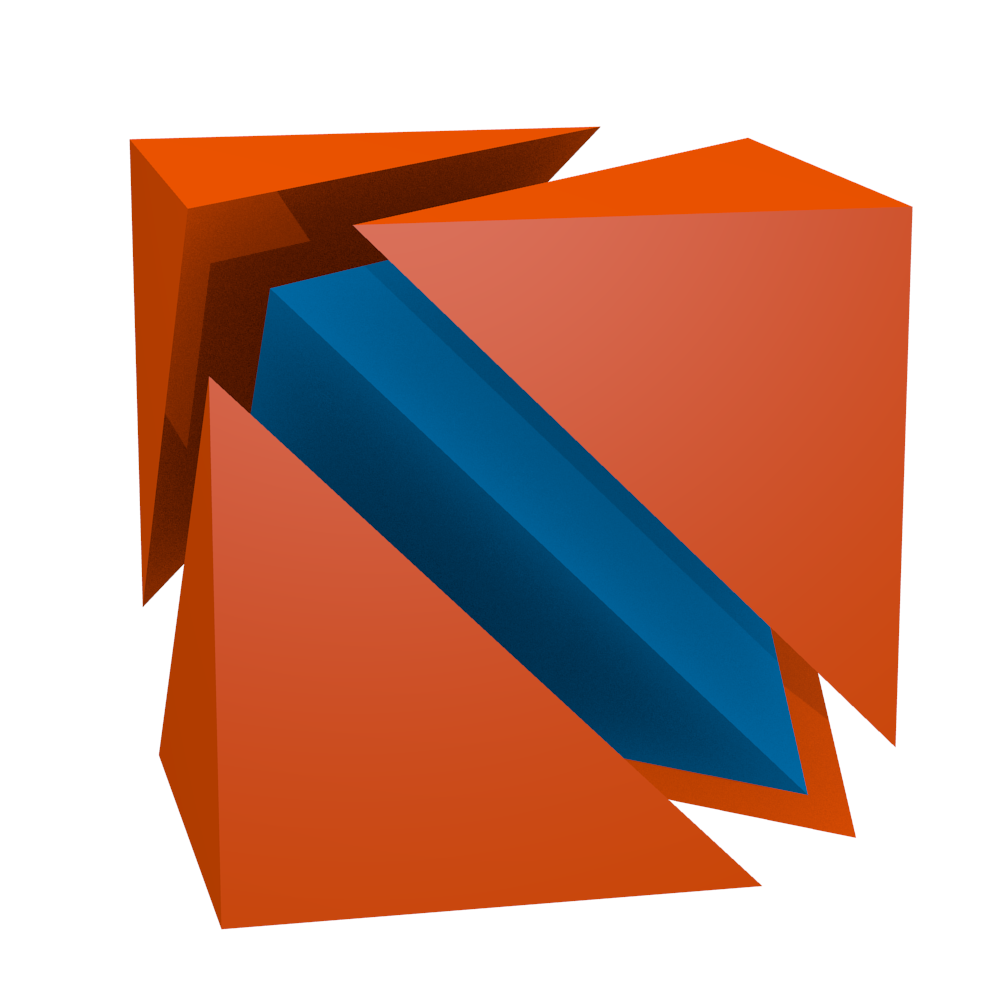
\includegraphics[width=0.4\textwidth]{images/fracture/hexahedron_to_tetrahedra.png}%
%     \caption{%
%         Illustration of how to divide a hexahedron into five tetraheda.%
%         \label{fig:hex_to_tetra}%
%     }%
% \end{figure}%
% %
% \begin{figure}[htpb]%
%     \centering%
%     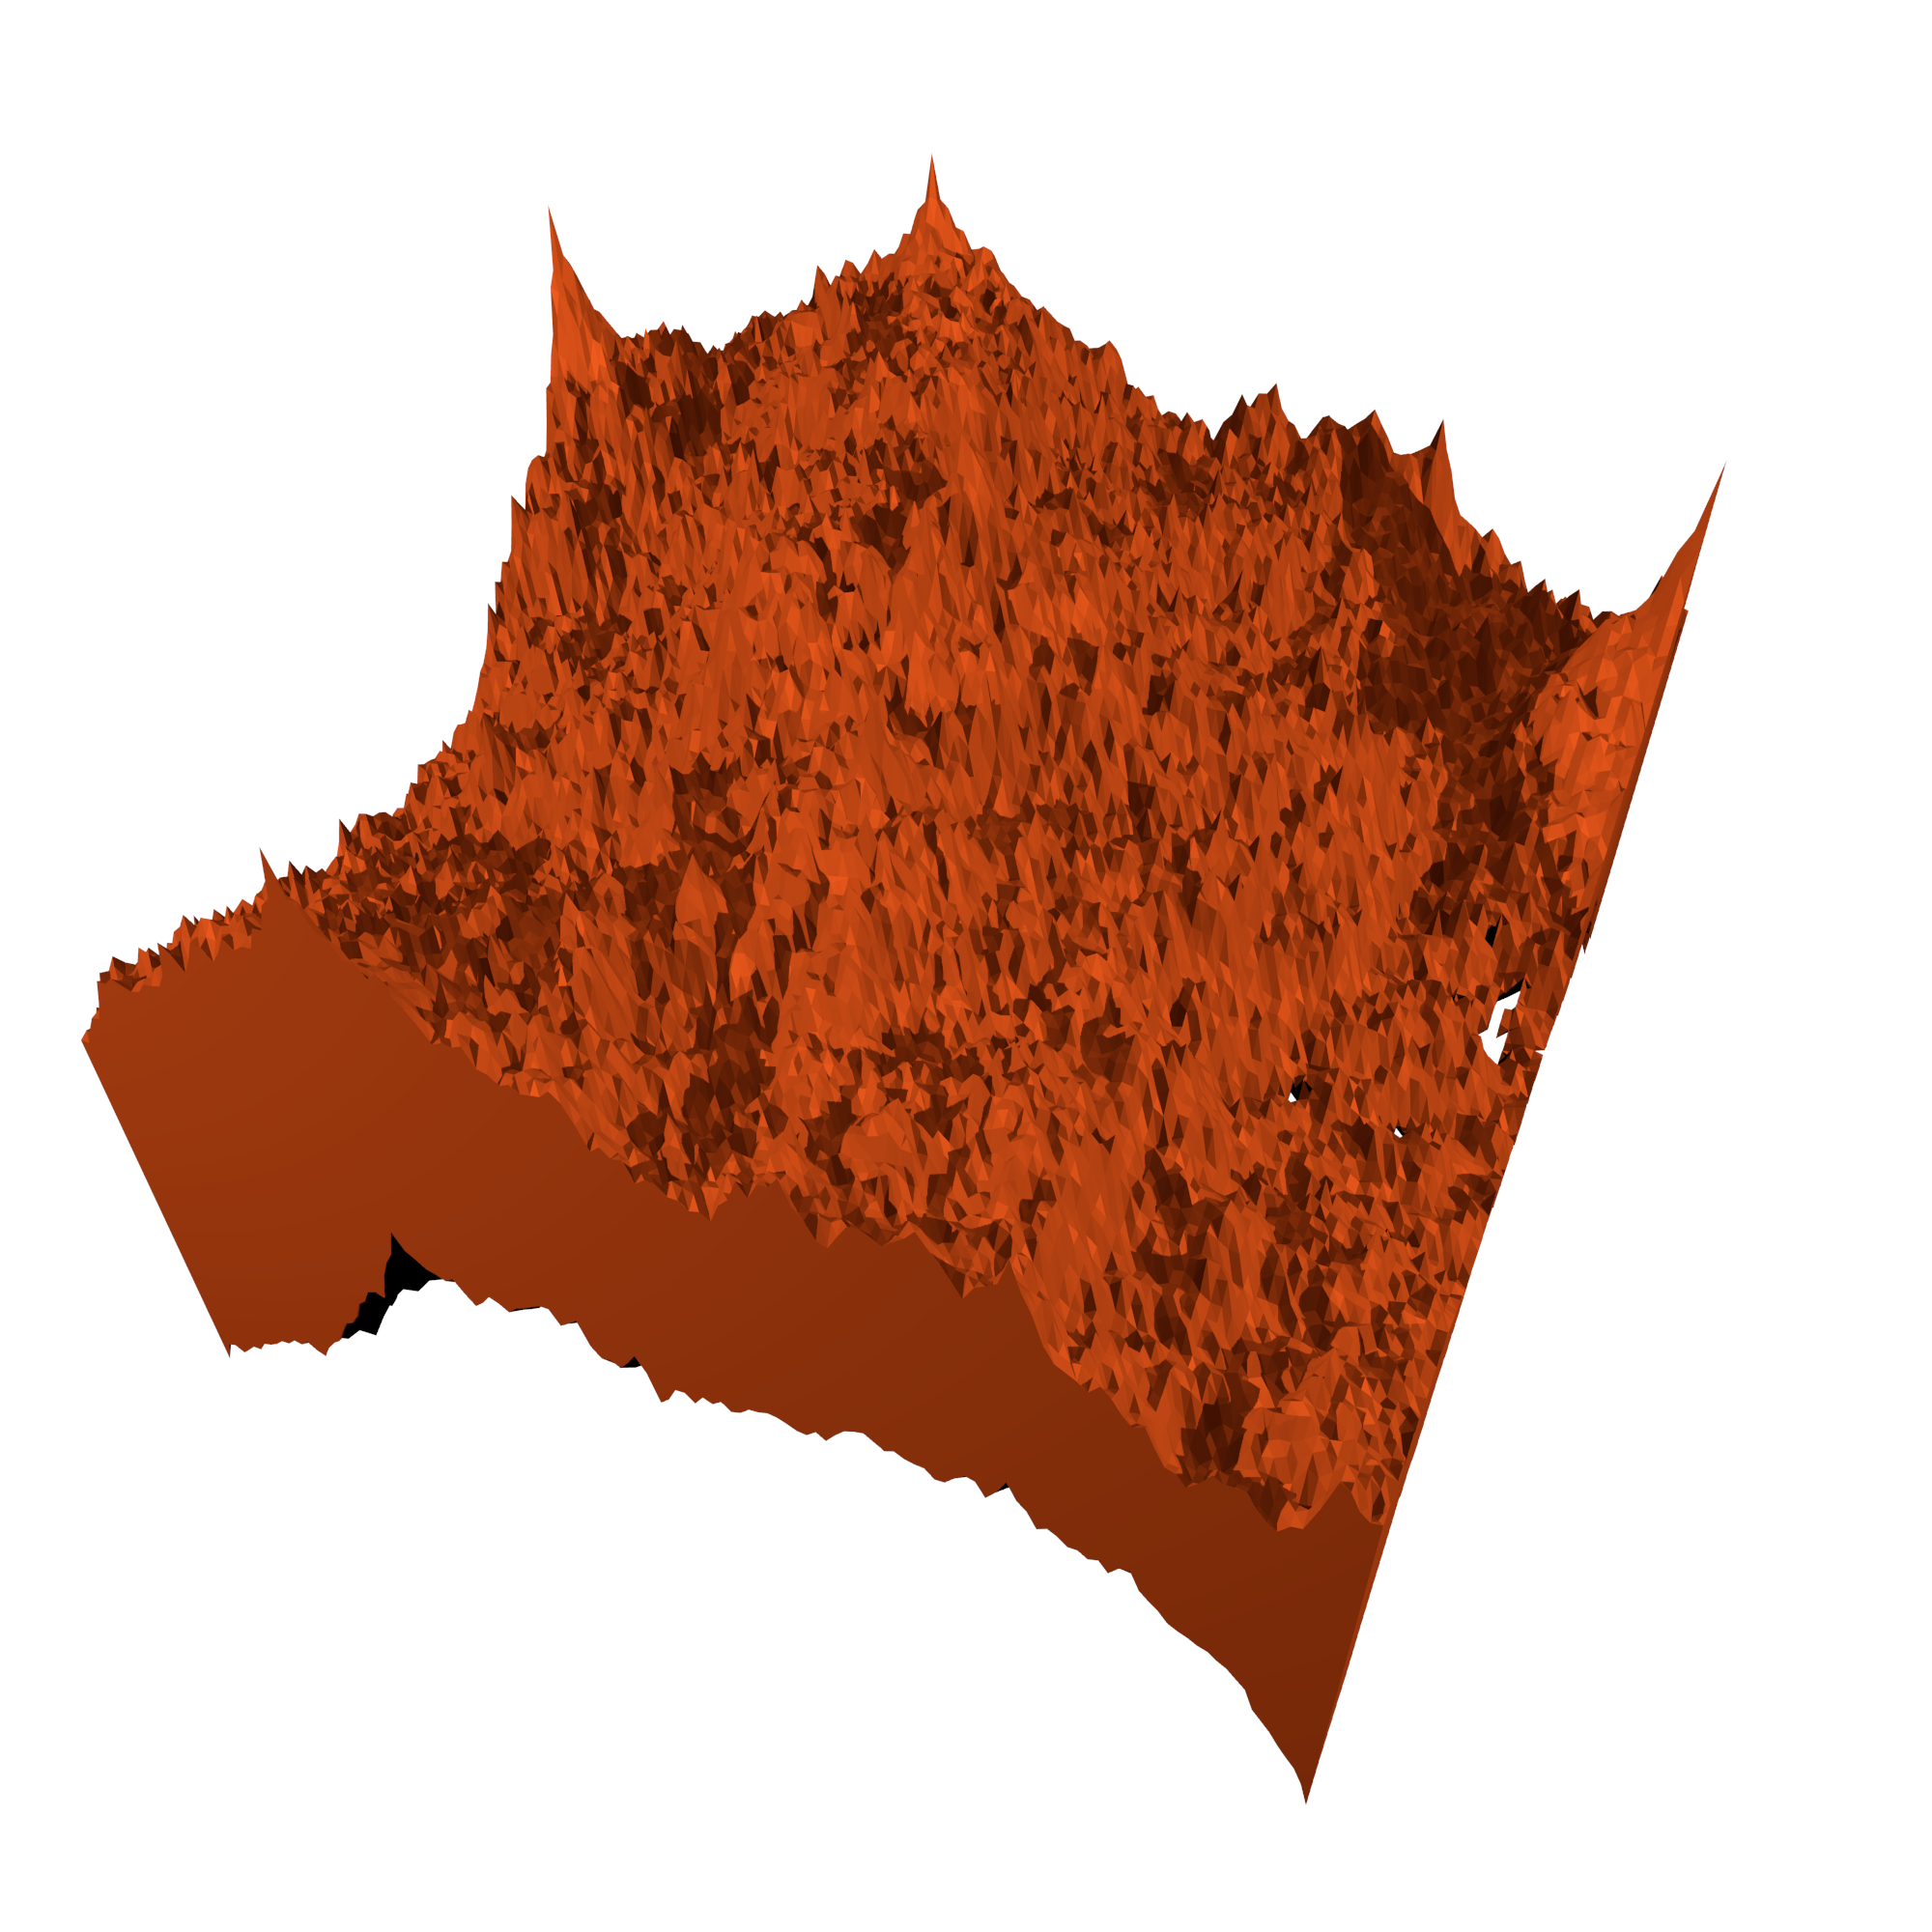
\includegraphics[width=0.6\textwidth]{images/fracture/fracture.png}%
%     \caption{%
%         A model of a fracture.%
%         \label{fig:fracture_model}%
%     }%
% \end{figure}%
%
\begin{figure}[htpb]%
    \centering%
    \setlength{\myfigwidth}{0.4\textwidth}%
%     \setlength{\mycaptionwidth}{0.3\textwidth}%
    \begin{subfigure}[b]{\myfigwidth}%
        \centering% % Need to center to get image centered over caption
        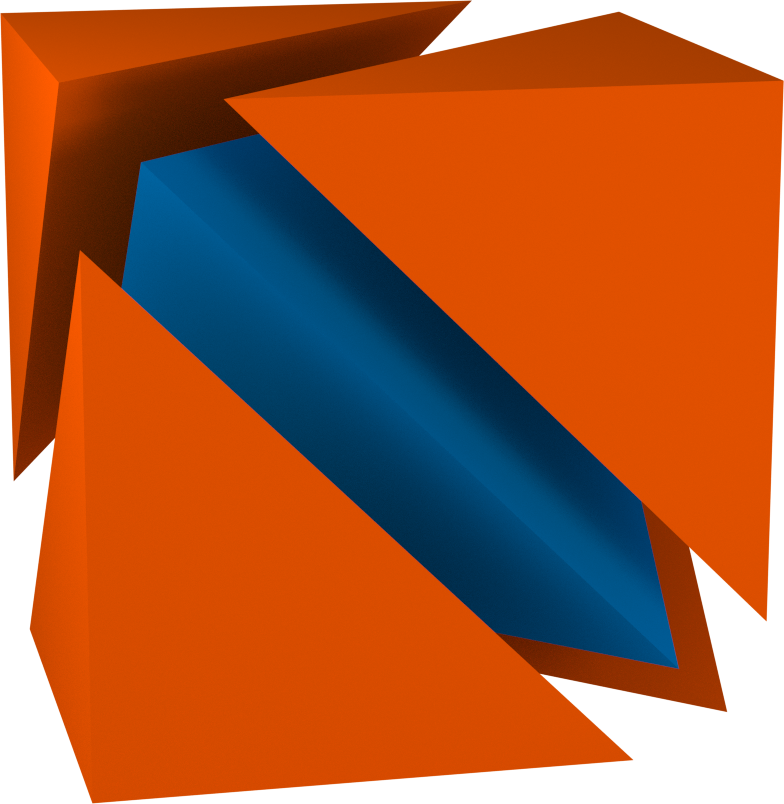
\includegraphics[width=0.6\textwidth]{images/fracture/hexahedron_to_tetrahedra01_cycles_n200_cropped.png}%
        \caption{Illustration of how to divide a convex hexahedron into five tetraheda.}%
        \label{fig:hex_to_tetra}%
    \end{subfigure}%
    \hspace{0.1\textwidth}%
    \begin{subfigure}[b]{\myfigwidth}%
        \centering%
        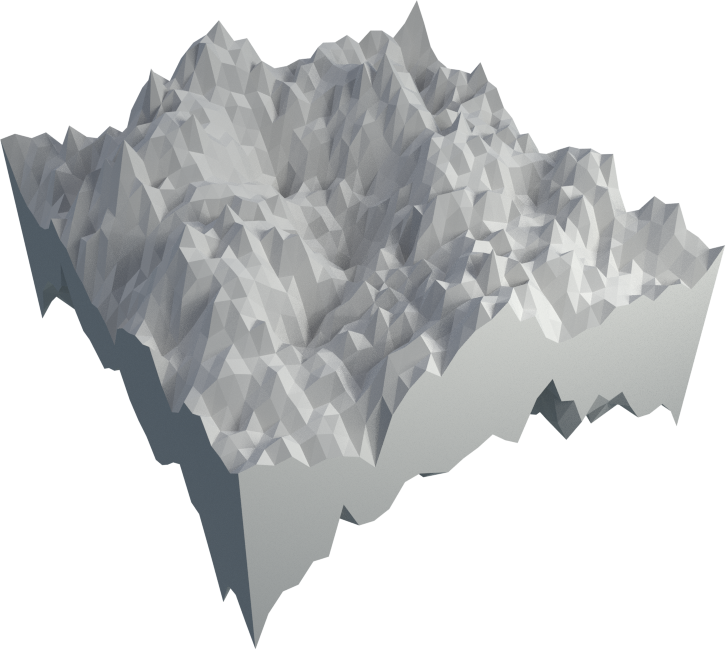
\includegraphics[width=\textwidth]{images/fracture/fracture05_n200_cropped.png}%
%         \includegraphics[width=\textwidth]{images/fracture/large_fracture04_300dpi_w20cm}%
        \caption{A random fracture made from two periodic surfaces.}%
        \label{fig:fracture_model}%
    \end{subfigure}%
\end{figure}%

\section{Surface area}
\section{Distance to nearest atom}
\begin{itemize}
    \item Fractals
    \item Fractional Brownian Motion
    \item The Hurst Exponent
\end{itemize}


